\documentclass[a4paper,11pt]{article}
\usepackage[T1]{fontenc}
\usepackage[utf8]{inputenc}
\usepackage{lmodern}
\usepackage{graphicx}
\usepackage{amsmath}
\usepackage{amsfonts}
\usepackage{amssymb}
\usepackage{mathtools}
\usepackage{epstopdf}

\DeclareMathOperator{\given}{\mid}

\begin{document}

\section*{HW0}

\begin{tabular*}{0.9\textwidth}{@{\extracolsep{\fill} } lll}
Jimmy Hold\"{o} & & Jared Karr\\
\aa\aa mmdd-xxxx & & 801120-4693\\
\it{gusholji@student.gu.se} & & \it{karr@student.chalmers.se}\\
\end{tabular*}

\section{Theoretical problems}
\subsection{Baye's rule}
Let $A\coloneqq\textit{has cancer}$ and $B\coloneqq\textit{positive test}$, then
\begin{align*}
P(A \given B) &= \frac{P(B \given A)\cdot P(A)}{P(B \given A)\cdot P(A)+P(B \given \neg A)\cdot P(\neg A)}  \\
              &= \frac{\frac{99}{100}\cdot\frac{1}{10\,000}}{\frac{99}{100}\cdot\frac{1}{10\,000}+\frac{1}{100}\cdot\frac{9999}{10\,000}} \\
              &= 0.0098
\end{align*}
meaning a patient who tests positive for cancer has less than $1\%$ chance of actually having it.

\subsection{Correlation and indepedence}
\clearpage
\section{Practical problems}
\subsection{Plotting normal distributed points}
\begin{figure}[h]
  \begin{center}
    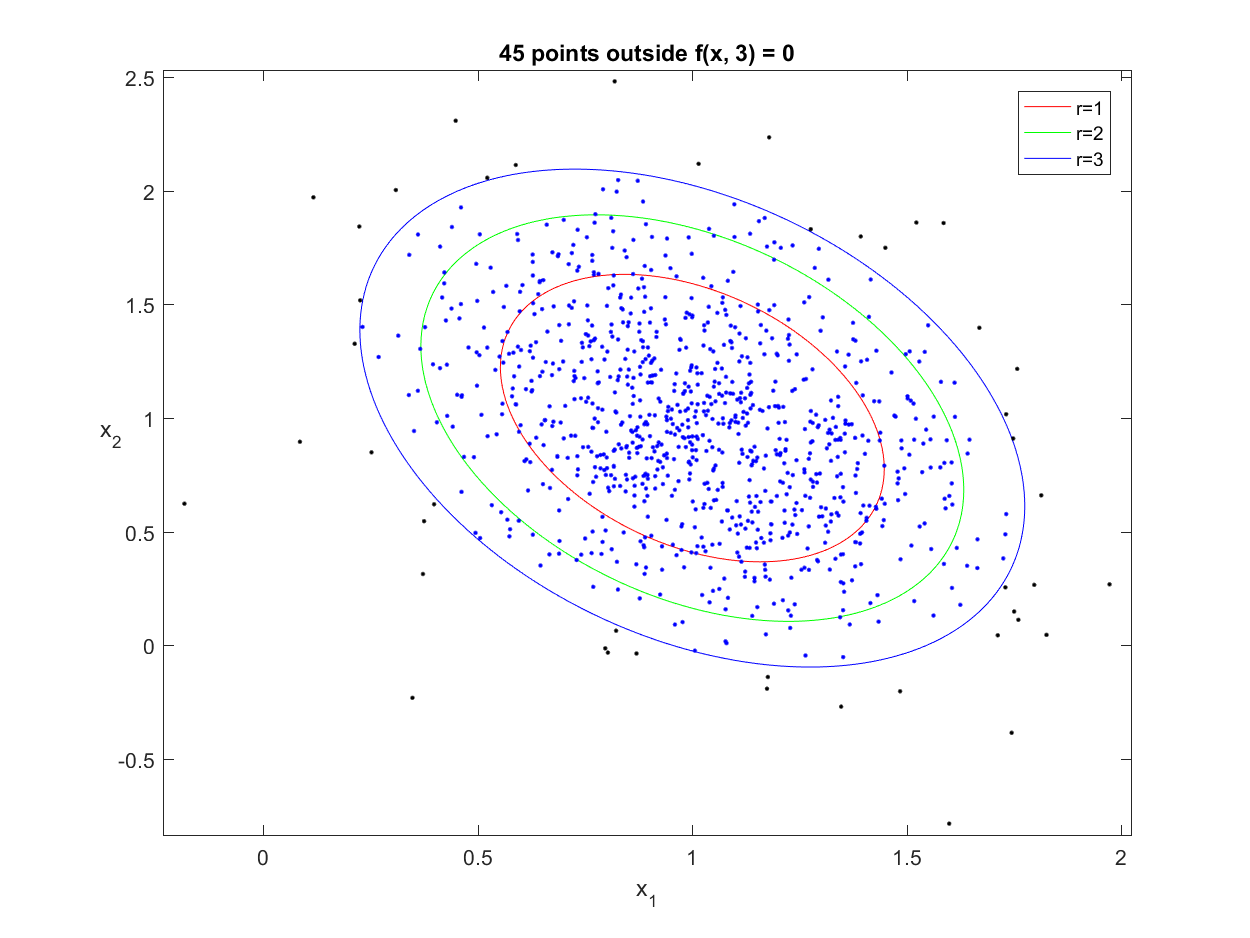
\includegraphics[width=\textwidth]{P2_1}
    \caption{}
    \label{fig:}
  \end{center}
\end{figure}
\clearpage
\subsection{Covariance and correlation}
\begin{figure}[h]
  \begin{center}
    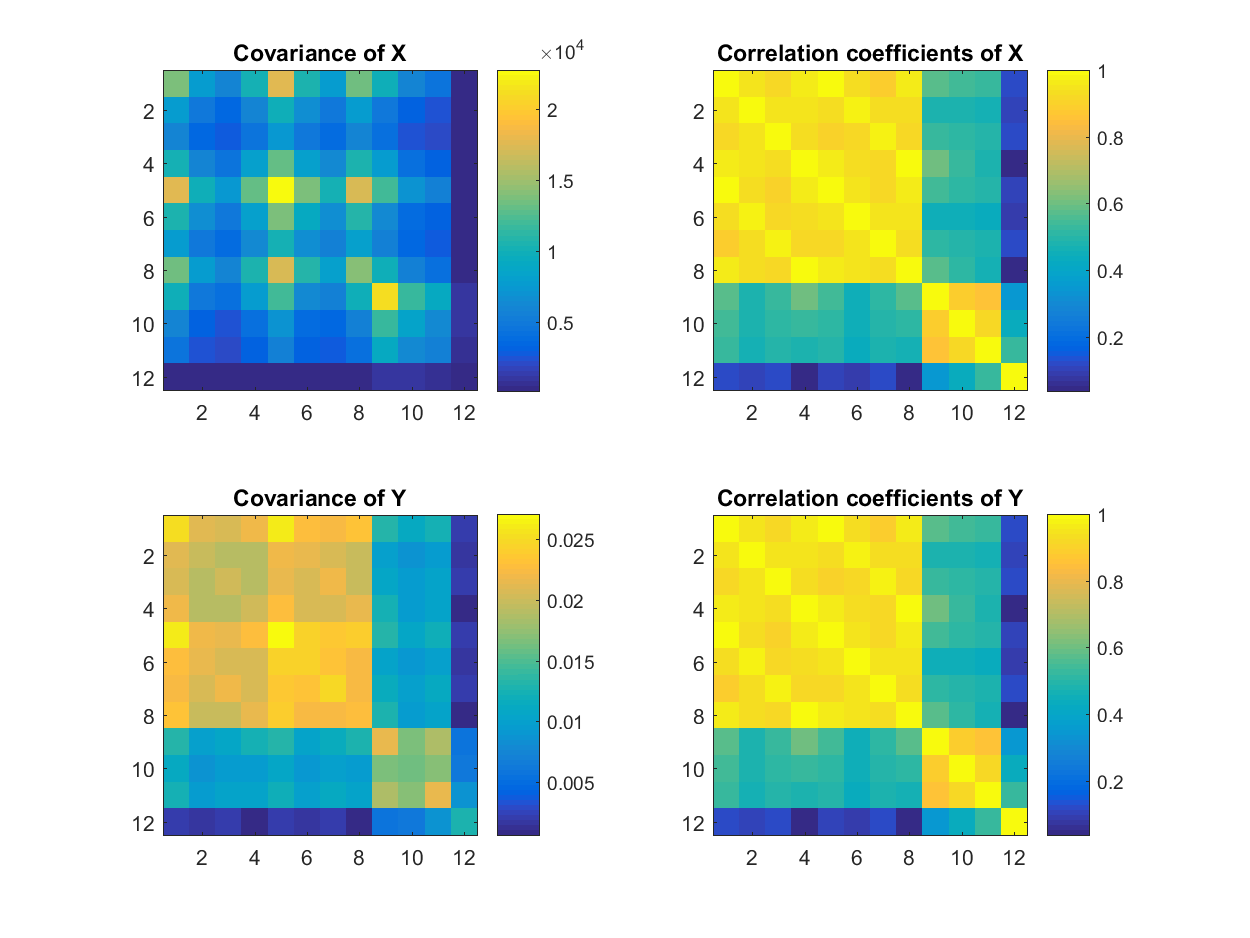
\includegraphics[width=\textwidth]{P2_2a}
    \caption{}
    \label{fig:}
  \end{center}
\end{figure}
\begin{figure}[h]
  \begin{center}
    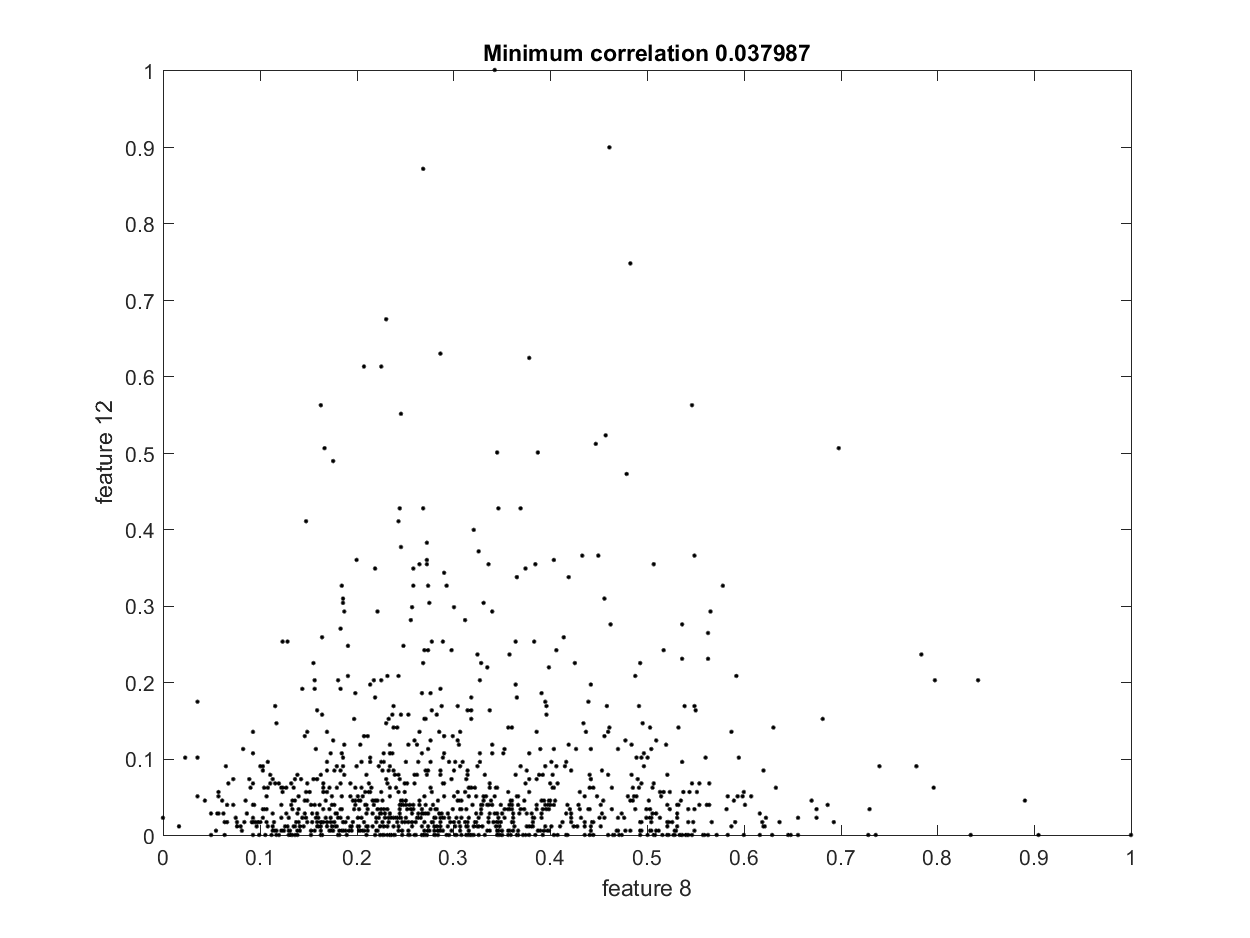
\includegraphics[width=\textwidth]{P2_2b}
    \caption{}
    \label{fig:}
  \end{center}
\end{figure}

\end{document}
